

\documentclass[twoside]{article}
\setlength{\oddsidemargin}{0.25 in}
\setlength{\evensidemargin}{-0.25 in}
\setlength{\topmargin}{-0.6 in}
\setlength{\textwidth}{6.5 in}
\setlength{\textheight}{8.5 in}
\setlength{\headsep}{0.75 in}
\setlength{\parindent}{0 in}
\setlength{\parskip}{0.1 in}

%
% ADD PACKAGES here:
%

\usepackage{amsmath,amsfonts,graphicx}

%
\newcounter{lecnum}
\renewcommand{\thepage}{\thelecnum-\arabic{page}}
\renewcommand{\thesection}{\thelecnum.\arabic{section}}
\renewcommand{\theequation}{\thelecnum.\arabic{equation}}
\renewcommand{\thefigure}{\thelecnum.\arabic{figure}}
\renewcommand{\thetable}{\thelecnum.\arabic{table}}

%
% The following macro is used to generate the header.
%
\newcommand{\lecture}[4]{
   \pagestyle{myheadings}
   \thispagestyle{plain}
   \newpage
   \setcounter{lecnum}{#1}
   \setcounter{page}{1}
   \noindent
   \begin{center}
   \framebox{
      \vbox{\vspace{2mm}
    \hbox to 6.28in { {\bf EE502 - Linear Systems Theory II
	\hfill Spring 2032} }
       \vspace{4mm}
       \hbox to 6.28in { {\Large \hfill Lecture #1 \hfill} }
       \vspace{2mm}
       \hbox to 6.28in { {\it Lecturer: #2 \hfill } }
      \vspace{2mm}}
   }
   \end{center}
   \markboth{Lecture #1}{Lecture #1}
}


\renewcommand{\cite}[2]{[#1]}
\def\beginrefs{\begin{list}%
        {[\arabic{equation}]}{\usecounter{equation}
         \setlength{\leftmargin}{2.0truecm}\setlength{\labelsep}{0.4truecm}%
         \setlength{\labelwidth}{1.6truecm}}}
\def\endrefs{\end{list}}
\def\bibentry#1{\item[\hbox{[#1]}]}

%Use this command for a figure; it puts a figure in wherever you want it.
%usage: \fig{NUMBER}{SPACE-IN-INCHES}{CAPTION}
\newcommand{\fig}[3]{
			\vspace{#2}
			\begin{center}
			Figure \thelecnum.#1:~#3
			\end{center}
	}
% Use these for theorems, lemmas, proofs, etc.
\newtheorem{theorem}{Theorem}[lecnum]
\newtheorem{lemma}[theorem]{Lemma}
\newtheorem{proposition}[theorem]{Proposition}
\newtheorem{claim}[theorem]{Claim}
\newtheorem{corollary}[theorem]{Corollary}
\newtheorem{definition}[theorem]{Definition}
\newenvironment{proof}{{\bf Proof:}}{\hfill\rule{2mm}{2mm}}

% **** IF YOU WANT TO DEFINE ADDITIONAL MACROS FOR YOURSELF, PUT THEM HERE:

\begin{document}
 
% Lecture Details
\lecture{12}{Assoc. Prof. M. Mert Ankarali}


\vspace{-12pt}

\section{State-Space Models of Dynamical Systems}

For a causal dynamical system, in order to compute output at a given
time, $t_0$ (or $k_o$ for DT systems), we need to know ``only'' the
input signal over $(-\infty , t_o]$ (or $(-\infty , k_o]$ for DT
systems). This requires a lot of data/information (indeed an infinite
amount of data), can we summarize it with something more manageable?
For example, using some latent variables stored in a vector, a.k.a. \textit{state-vector}.

\textbf{State property of DT state-space models:} 
Given the state vector $x[k_0]$ and input $u[k_0]$ at an arbitrary time $k_0$, 
we can compute the the present output, $y[k_0]$, and next state
$x[k_0+1]$.

\textbf{State property of CT state-space models:} Given the initial time,
$t_0$ and state $x(t_0)$ and input $u(t)$ for $t_0 \leq t \leq t_f$ (with
$t_0 \ \& \ t_f$ arbitrary), we can compute the output $y(t)$ for 
$t_0 \leq t \leq t_f$ and the state $x(t)$ for  $t_0 \leq t \leq t_f$. 

In other words $x(t_0)$ (and $x[k_0]$ for DT systems) summarizes the
whole input history, $t\in(-\infty , t_0)$ (or $k \in (-\infty ,
k_0)$) in a compact (most probably \textit{finite-dimensional}) memory package,
for the purpose of predicting the future output (and states)

Note that neither definition is limited to LTI state-space models. 
Nonlinear and time-varying state-space models also are based on this 
definition. CT state-property is more and also applies for DT state-space models. 

Note that the choice of state variables is not unique (and there exist infinite possible of \textit{realizations}); however, there are some options that are preferable to others (minimal representations, canonical forms, practical benefits, etc.). When a state-space representation includes the minimum possible number of state variables, the representation is called minimal. 

\vspace{-12pt}

\subsection{State-Space Representations of LTI, LTV, \& Non-Linear
  Dynamical Systems}

\textbf{LTI Systems}

State-space representation of a (causal \& finite-dimensional) LTI CT system is given by
%
\begin{align*}
  \mathrm{Let} \ x(t) &\in \mathbb{R}^n \ , \ y(t) \in \mathbb{R}^m \ ,\  u(t) \in
  \mathbb{R}^r , \\
  \dot{x}(t) &= A x(t) + B u(t) , \\
  y(t) &= C x(t) + D u(t) , \\
  \mathrm{where} \ A &\in \mathbb{R}^{n \times n} \ , \ 
    B \in \mathbb{R}^{n \times r} \ ,\  C \in \mathbb{R}^{m \times n} \ , \ D \in \mathbb{R}^{m \times r}
\end{align*}
%
State-space representation of a (causal \& finite dimensional) LTI DT system is given by
%
\begin{align*}
  \mathrm{Let} \ x[k] &\in \mathbb{R}^n \ , \ y[k] \in \mathbb{R}^m \ ,\  u[k] \in
  \mathbb{R}^r , \\
  x[k+1] &= G x[k] + H u[k] , \\
  y[k] &= C x[k] + D u[k] , \\
  \mathrm{where} \ G &\in \mathbb{R}^{n \times n} \ , \ 
    H \in \mathbb{R}^{n \times r} \ ,\  C \in \mathbb{R}^{m \times n} \ , \ D \in \mathbb{R}^{m \times r}
\end{align*}
%

\textbf{LTV Systems}

State-space representation of a (causal \& finite dimensional) LTV CT system is given by
%
\begin{align*}
  \mathrm{Let} \ x(t) &\in \mathbb{R}^n \ , \ y(t) \in \mathbb{R}^q \ ,\  u(t) \in
  \mathbb{R}^p , \\
  \dot{x}(t) &= A(t) x(t) + B(t) u(t) , \\
  y(t) &= C(t) x(t) + D(t) u(t) , \\
  \mathrm{where} \ A(t) &\in \mathbb{R}^{n \times n} \ , \ 
    B(t) \in \mathbb{R}^{n \times p} \ ,\  C(t) \in \mathbb{R}^{q \times n} \ , \ D(t) \in \mathbb{R}^q
\end{align*}
%
State-space representation of a (causal \& finite dimensional) LTV DT system is given by
%
\begin{align*}
  \mathrm{Let} \ x[n] &\in \mathbb{R}^n \ , \ y[n] \in \mathbb{R}^q \ ,\  u[n] \in
  \mathbb{R}^p , \\
  x[n+1] &= A[n] x[n] + B[n] u[n] , \\
  y[n] &= C[n] x[n] + D[n] u[n] , \\
  \mathrm{where} \ A[n] &\in \mathbb{R}^{n \times n} \ , \ 
    B[n] \in \mathbb{R}^{n \times p} \ ,\  C[n] \in \mathbb{R}^{q
                          \times  n} \ , \ D[n] \in \mathbb{R}^q
\end{align*}

\textbf{Non-Linear Systems}

State-space representation of a (causal \& finite dimensional) non-linear CT system is given by
%
\begin{align*}
  \mathrm{Let} \ x(t) &\in \mathbb{R}^n \ , \ y(t) \in \mathbb{R}^q \ ,\  u(t) \in
  \mathbb{R}^p , \\
  \dot{x}(t) &= F(x(t),u(t)) , \\
  y(t) &= H(x(t),u(t)) , 
\end{align*}
%
State-space representation of a (causal \& finite dimensional) non-linear DT system is given by
%
\begin{align*}
  \mathrm{Let} \ x[n] &\in \mathbb{R}^n \ , \ y[n] \in \mathbb{R}^q \ ,\
                        u[n] \in \mathbb{R}^p , \\
  x[n+1] &= F(x[n],u[n]) , \\
  y[n] &= H(x[n],u[n]) , 
\end{align*}

\subsection{Example CT and DT System Models}

\textbf{Ex 1: Series RLC Circuit}

Given than input is $u(t) = V_s(t)$ and output os $y(t) = V_C(t)$,
first find an ODE description of the given dynamical circuit. 

  \begin{minipage}[h]{0.5\linewidth}
    \begin{center}
      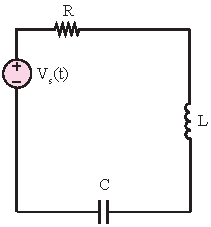
\includegraphics[width=0.75\textwidth]{RLC}
    \end{center}
  \end{minipage}
  \begin{minipage}[h]{0.5\linewidth}
    \begin{center}
    {\large
  \begin{align*}
  	V_L + V_R + V_C &= V_s(t)
	\\
	L \frac{d I}{dt} + R I + V_C &= V_s(t)
	\\
	L \frac{d }{dt} \left( C \frac{d V_C}{dt} \right) + R  \left( C \frac{d V_C}{dt} \right) + V_C &= V_s(t)
	\\
	LC \ \ddot{V}_C + RC \ \dot{V_C} + V_C &= V_s(t)
	\\
	\ddot{y} + \frac{R}{L} \dot{y} + \frac{1}{LC} y &= \frac{1}{LC} u
  \end{align*}
  }
    \end{center}
  \end{minipage}

Now, find the transfer function representation of the system for the given input--output pair.
%
\begin{align*}
	\mathcal{L} \left\lbrace \ddot{y} + \frac{R}{L} \dot{y} + \frac{1}{LC} y  \right\rbrace 
	&= \mathcal{L} \left\lbrace \frac{1}{LC} u  \right\rbrace
	\\
	s^2 Y(s) + s \frac{R}{L} Y(s) + \frac{1}{LC} Y(s) &=  \frac{1}{LC} U(s) \\
	G(s) = \frac{Y(s)}{U(s)} &= \frac{\frac{1}{LC} }{s^2 + \frac{R}{L} s + \frac{1}{LC} }
\end{align*}
%
Find a state-space representation of the system.
%
Let $x = \left[ \begin{array}{c} x_1 \\ x_2 \end{array} \right] = \left[ \begin{array}{c} y \\ \dot{y} \end{array} \right]$, then 
%
\begin{align*}
	\dot{x_1} &= x_2 \\
	\dot{x_2} &= -\frac{1}{LC} x_1 - \frac{R}{L} x_2 + \frac{1}{LC} u
\end{align*}
%
If we put the equations in state-space form, we obtain
%
\begin{align*}
 \dot{x} &= \left[  \begin{array}{cc} 0 & 1 \\ -\frac{1}{LC} &  -\frac{R}{L}  \end{array} \right] x 
 +  \left[  \begin{array}{c} 0 \\ \frac{1}{LC} \end{array} \right] u
 \\
 y &= \left[  \begin{array}{cc} 1 & 0 \end{array} \right] x 
\end{align*}
%
where
%
\begin{align*}
 A = \left[  \begin{array}{cc} 0 & 1 \\ -\frac{1}{LC} &  -\frac{R}{L}  \end{array} \right] \quad , \
 B = \left[  \begin{array}{c} 0 \\ \frac{1}{LC} \end{array} \right]  \quad , \
 C = \left[  \begin{array}{cc} 1 & 0 \end{array} \right] \quad , \
 D = 0
\end{align*}

Now let, $z = \left[ \begin{array}{c} z_1 \\ z_2 \end{array} \right] =
\left[ \begin{array}{c} V_C \\ I \end{array} \right]$, then 
%
\begin{align*}
	\dot{z_1} &= \frac{1}{C} z_2 \\
	\dot{z_2} &= -\frac{1}{L} z_1 - \frac{R}{L} z_2 + \frac{1}{L} u
\end{align*}
%
If we put the equations in state-space form, we obtain
%
\begin{align*}
 \dot{z} &= \left[  \begin{array}{cc} 0 & \frac{1}{C} \\ -\frac{1}{L} &  -\frac{R}{L}  \end{array} \right] z 
 +  \left[  \begin{array}{c} 0 \\ \frac{1}{L} \end{array} \right] u
 \\
 y &= \left[  \begin{array}{cc} 1 & 0 \end{array} \right] z
\end{align*}
%
\textbf{Home practice:} Comment on the similarities and differences between two representations.

\newpage

\textbf{Ex 2: State-Space Realization of a Third Order FIR Systems}

A third order FIR (Finite impulse response) filter has the following
difference equation and transfer function
%
\begin{align*}
y[k] &= b_0 u[k] + b_1 u[k-1] + b_2 u[k-2] + b_3 u[k-3] \\ 
Y(z) &= \left( b_0 + b_1 z^{-1} + b_2 z^{-2} + b_3 z^{-3} \right) U(z)
\end{align*}
%
From inspection it is easy to see that we need at least three memory (unit delay) 
blocks to construct a the realization. Fig.~\ref{fig:FIR} also 
provides the block-diagram realization of a third order FIR filter.
%
\begin{figure}[h]
    \centering
      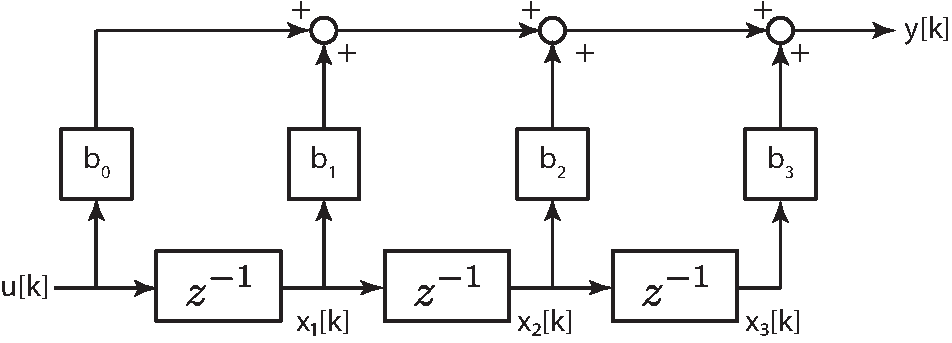
\includegraphics[width=0.75\textwidth]{FIR}
    \caption{Block diagram realization of a third order FIR system}
        \label{fig:FIR}
\end{figure}
%
Let $x[k] = \left[ \begin{array}{c} x_1[k] \\ x_2[k] \\ x_3[k]
\end{array} \right] = \left[ \begin{array}{c} u[k-1] \\ u[k-2] \\
                               u[k-3] \end{array} \right] $ , then 
%
\begin{align*}
 x[k+1] &= \left[  \begin{array}{ccc} 0 & 0 & 0 \\ 1 & 0 & 0 \\ 0 & 1 & 0 \end{array} \right] x[k] 
 +  \left[  \begin{array}{c} 1 \\ 0 \\ 0  \end{array} \right] u[k]
 \\
 y &= \left[  \begin{array}{ccc} b_1 & b_2 & b_3 \end{array} \right] x[k] + [b_0] u[k]
\end{align*}
%

\vspace{6pt}

\textbf{Ex 3: Pendulum}

Given than input is $u(t) = \tau(t)$ and output os $y(t) = \theta(t)$,
find a state-space model of the pendulum dynamics.

  \begin{minipage}[h]{0.4\linewidth}
    \begin{center}
      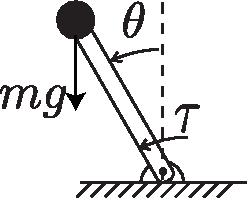
\includegraphics[width=0.75\textwidth]{pendulum}
    \end{center}
  \end{minipage}
  \begin{minipage}[h]{0.6\linewidth}
    \begin{center}
    {\large
  \begin{align*}
       m l^2 \ddot{\theta} &= \tau(t) + m g l \sin(\theta)
	\\
	\mathrm{Let} \ x &= \left[ \begin{array}{c} \theta \\ \dot{\theta} \end{array} \right] 
	\\
	\dot{x} &= \left[ \begin{array}{c} x_2 \\ \frac{g}{l}
                           \sin(x_1) \end{array} \right] +
    \left[ \begin{array}{c} 0 \\ \frac{1}{m l^2} \end{array} \right] u
	\\
        y &= \left[ \begin{array}{cc} 1 & 0 \end{array} \right] x
	\\
       f(x,u) &= \left[ \begin{array}{c} x_2 \\ \frac{g}{l}
                           \sin(x_1) + \frac{1}{m l^2} u \end{array} \right]  
  \end{align*}
  }
    \end{center}
  \end{minipage}

\newpage

\textbf{Ex 4: Predator-Prey Model}
%
Consider an island populated primarily by goats and foxes. Goat's
survive and breed by consuming the island's sources, while foxes
survive and breed by consuming goats. To build a DT state-space model
(based on behavioral observations) let's define following state
variables
%
  \begin{align*}
    x_1[k] : \# \mathrm{goats} \\
    x_2[k] : \# \mathrm{foxes} \\
  \end{align*}
%
State-equation for the population of goats can be modeled as
%
  \begin{align*}
    x_1[k+1] = g x_1[k] - c_{fg} x_1[k] x_2[k] 
  \end{align*}
%
where $g > 1$ (which models geometric growth rate of gots), and
$c_{fg} > 0$. Note that $- c_{fg} x_1[k] x_2[k] $ models the negatif
effect of fox population on goat population. On the other hand 
state-equation for the population of fox can be modeled as
%
  \begin{align*}
    x_2[k+1] = f x_2[k] + c_{gf} x_1[k] x_2[k] 
  \end{align*}
%
where $0 < f < 1$ (which models geometric decay rate of foxes), and
$c_{gf} > 0$. Note that $c_{gf} x_2[k] x_1[k] $ models the pozitif
effect of goat population on fox population. If we combine both of the 
state equations we obtain
%
\begin{align*}
	x[k+1] &= \left[ \begin{array}{c} g x_1[k+1] - c_{fg} x_1[k] x_2[k]   \\ 
                          f x_2[k] + c_{gf} x_1[k] x_2[k]  \end{array} \right] 
\end{align*}
%
Note that as constructed this is an autonomous dynamical system (no
external input)

\subsection{Linearization of Non-linear Dynamical Systems}

Consider a non-linear CT dynamical system represented in state-space form
%
\begin{align*}
  \mathrm{Let} \ x(t) &\in \mathbb{R}^n \ , \ y(t) \in \mathbb{R}^q \ ,\  u(t) \in
  \mathbb{R}^p , \\
  \dot{x}(t) &= F(x(t),u(t)) , \\
  y(t) &= H(x(t),u(t)) , 
\end{align*}
%
Suppose that we are intersted in finding an approximate linear
dynamical system model around a nominal point (equilibrium),
$(x_o,u_o,y_o))$ that solves the equation constraints, i.e.
%
\begin{align*}
  0 &= F(x_0,u_o) , \\
  y(t) &= H(x_o,u_o) , 
\end{align*}
%
Since we are intersted in the dynamics around the nominal solution, we
define set of ``small'' \textit{perturbation} variables; $\delta x(t)
= x(t) - x_o \ , \ \delta u(t) = u(t) - u_o \ \& \ \delta y(t) = y(t)
- x_o \ , \ $. If we perform a (multivariate) first order Taylor
series expansion, we can find the linerized state-space model as
%
\begin{align*}
  \dot{\delta x} &\approx \left( \left[ \frac{\partial F(x,u)}{\partial x}
                      \right]_{(x_o,u_o)} \right) \delta x + \left( \left[ \frac{\partial F(x,u)}{\partial u}
                      \right]_{(x_o,u_o)} \right) \delta u  , \\
  \delta y  &\approx \left( \left[ \frac{\partial H(x,u)}{\partial x}
                      \right]_{(x_o,u_o)} \right) \delta x + \left( \left[ \frac{\partial H(x,u)}{\partial u}
                      \right]_{(x_o,u_o)} \right) \delta u , 
\\ 
&\mathrm{where}
\\
A &= \left( \left[ \frac{\partial F(x,u)}{\partial x}
                      \right]_{(x_o,u_o)} \right) \ , \ B = \left( \left[ \frac{\partial F(x,u)}{\partial u}
                      \right]_{(x_o,u_o)} \right)
\\
C &= \left( \left[ \frac{\partial H(x,u)}{\partial x}
                      \right]_{(x_o,u_o)} \right) \ , \ D = \left( \left[ \frac{\partial H(x,u)}{\partial u}
                      \right]_{(x_o,u_o)} \right)
\end{align*}
%

\textbf{Ex 3-2: Linearization(s) of the Pendulum Model}

Compute the approximate linear model of the pendulum around $(x,u) =
\left( \left[ \begin{array}{c} 0 \\ 0 \end{array} \right] , 0 \right)$
%
\begin{align*}
A &= \left( \left[ \frac{\partial F(x,u)}{\partial x}
                      \right]_{(x_o,u_o)} \right) =
                    \left[ \begin{array}{cc} 0 & 1 \\ g/l & 0 \end{array}  \right]
\ , \ B = \left( \left[ \frac{\partial F(x,u)}{\partial u}
                      \right]_{(x_o,u_o)} \right) =
                                                            \left[ \begin{array}{c}
                                                                     0
                                                                     \\
                                                                     \frac{1}{m
                                                                     l^2}  \end{array}  \right]
\ , \
C &= \left[ \begin{array}{cc} 1 & 0 \end{array}  \right]
\end{align*}
%
Compute the approximate linear model of the pendulum around $(x,u) =
\left( \left[ \begin{array}{c} \pi \\ 0 \end{array} \right] , 0 \right)$
%
\begin{align*}
A &= \left( \left[ \frac{\partial F(x,u)}{\partial x}
                      \right]_{(x_o,u_o)} \right) =
                    \left[ \begin{array}{cc} 0 & 1 \\ -g/l & 0 \end{array}  \right]
\ , \ B = \left( \left[ \frac{\partial F(x,u)}{\partial u}
                      \right]_{(x_o,u_o)} \right) =
                                                            \left[ \begin{array}{c}
                                                                     0
                                                                     \\
                                                                     \frac{1}{m
                                                                     l^2}  \end{array}  \right]
\ , \
C &= \left[ \begin{array}{cc} 1 & 0 \end{array}  \right]
\end{align*}
%
Compute the approximate linear model of the pendulum around $(x,u) =
\left( \left[ \begin{array}{c} -\pi/2 \\ 0 \end{array} \right] , m g l \right)$
%
\begin{align*}
A &= \left( \left[ \frac{\partial F(x,u)}{\partial x}
                      \right]_{(x_o,u_o)} \right) =
                    \left[ \begin{array}{cc} 0 & 1 \\ 0 & 0 \end{array}  \right]
\ , \ B = \left( \left[ \frac{\partial F(x,u)}{\partial u}
                      \right]_{(x_o,u_o)} \right) =
                                                            \left[ \begin{array}{c}
                                                                     0
                                                                     \\
                                                                     \frac{1}{m
                                                                     l^2}  \end{array}  \right]
\ , \
C &= \left[ \begin{array}{cc} 1 & 0 \end{array}  \right]
\end{align*}

Now suppuse that we are intersted in finding an apprximate liner
dynamical system model for a non-linear discrete-time dynamical
system. Actually the process is exactly same (since we are still
utilizing Taylor series expansion around a nominal point), except that 
the definition of nominal solution is different. Let's assume that 
a nominal point (equilibrium), $(x_o,u_o,y_o))$ solves the equation
constraints of the non-linear discrete-time dynamical system, then 
we know that
\begin{align*}
  x_o &= F(x_o,u_o) , \\
  y_o &= H(x_o,u_o) , 
\end{align*}
%
Cumputation of state-space matrices and definition of perturbation
variables are completely same for the CT case. 
%

\vspace{12pt}

\textbf{Ex 4-2: Linearization of the Predator-Prey Model}

Let $[g , f , c_{fg} , c_{gf}] = [2 , 0.5 , 0.1 , 0.05]$, first compute the
equilibrium point of the dynamical system
%
\begin{align*}
	\left[ \begin{array}{c} \bar{x}_{1} \\ \bar{x}_{2} \end{array} \right]  &=
\left[ \begin{array}{c} 2 \bar{x}_1 - 0.1 \bar{x}_1 \bar{x}_2   \\ 
 0.5 \bar{x}_2 + 0.05 \bar{x}_1 \bar{x}_2  \end{array} \right] \
  \rightarrow \ x_0 = \left[ \begin{array}{c} 10 \\ 10 \end{array} \right] 
\end{align*}
%
Now linarize the dynamics around the equilibrium and derive the
approximate DT linear state-space representation
%
\begin{align*}
A &= \left( \left[ \frac{\partial F(x)}{\partial x}
                      \right]_{(x_o)} \right) =
    \left[ \begin{array}{cc} 2 - 1 & 
             - 1 \\ 
                          0.5 
           & 
             0.5 + 0.5
\end{array} \right]  =
                    \left[ \begin{array}{cc} 1 & -1 \\ 0.5 & 1 \end{array}  \right]
\end{align*}

\newpage

Let's go back to non-linear CT time dynamical models. Sometimes, 
we want to obtain a \textit{Linear} dynamical system model 
around a nominal trajecotry (not a point) which still satisfies the
constraints of the dynamical system. In such a case nominal solution 
takwa the form $(x_o(t),u_o(t),y_o(t)))$ ans still satisfies the equation constraints, i.e.
%
\begin{align*}
  \dot{x_o}(t) &= F(x_o(t),u_o(t)) \ , \  y_o(t) = H(x_o(t),u_o(t)) , \ \forall
                                        t \in \mathbb{R}
\end{align*}
%
We define set of ``small'' \textit{perturbation} variables in a
similar way; $\delta x(t)
= x(t) - x_o(t) \ , \ \delta u(t) = u(t) - u_o(t) \ \& \ \delta y(t) = y(t)
- y_o(t)$. Indeed formulation of the (multivariate) first order Taylor
series expansion is (almost) exactly same, and we can find the linerized state-space model as
%
\begin{align*}
  \dot{\delta x}(t) &\approx \left( \left[ \frac{\partial F(x,u)}{\partial x}
                      \right]_{(x_o(t),u_o(t))} \right) \delta x + \left( \left[ \frac{\partial F(x,u)}{\partial u}
                      \right]_{(x_o(t),u_o(t))} \right) \delta u(t)  , \\
  \delta y(t)  &\approx \left( \left[ \frac{\partial H(x,u)}{\partial x}
                      \right]_{(x_o(t),u_o(t))} \right) \delta x(t) + \left( \left[ \frac{\partial H(x,u)}{\partial u}
                      \right]_{(x_o(t),u_o(t))} \right) \delta u(t) , 
\\ 
&\mathrm{where}
\\
A(t) &= \left( \left[ \frac{\partial F(x,u)}{\partial x}
                      \right]_{(x_o(t),u_o(t))} \right) \ , \ B(t) = \left( \left[ \frac{\partial F(x,u)}{\partial u}
                      \right]_{(x_o(t),u_o(t))} \right)
\\
C(t) &= \left( \left[ \frac{\partial H(x,u)}{\partial x}
                      \right]_{(x_o(t),u_o(t))} \right) \ , \ D(t) = \left( \left[ \frac{\partial H(x,u)}{\partial u}
                      \right]_{(x_o(t),u_o(t))} \right)
\end{align*}
%
Note that in such a case state-space matrices (almost surely) potentially becomes
time-dependent and hence linearitzation leads to a LTV
(Linear-Time-Varying) state-space model. 

\vspace{12pt}

\textbf{Ex 3-3: Linearization(s) of the Pendulum Model Around a Trajectory}

Let's go back to the simple pendulum model. We want to ``control'' the
system such that it rotates with a constant angular velocity and
analyze the dynamics around the nominal trajectory. In that
respect nominal trajectory for the state variables can take the
following form
%
\begin{align*}
x_o(t) = \left[ \begin{array}{c} \theta_o(t) \\ \dot{\theta}_o(t) \end{array}
  \right] = \left[ \begin{array}{c} t \\ 1 \end{array}
  \right] 
\end{align*}
%
Compute the nominal solution for the input that satisfies the nominal
state-trajectories
%
%
\begin{align*}
u_0(t) = m g l \sin(t)
\end{align*}
%

Compute the approximate linear model of the pendulum around $(x_o(t),u_o(t)) $
%
\begin{align*}
A(t) &= \left( \left[ \frac{\partial F(x,u)}{\partial x}
                      \right]_{(x_o,u_o)} \right) =
                    \left[ \begin{array}{cc} 0 & 1 \\ g/l \cos(t) & 0 \end{array}  \right]
\ , \ B = \left( \left[ \frac{\partial F(x,u)}{\partial u}
                      \right]_{(x_o,u_o)} \right) =
                                                            \left[ \begin{array}{c}
                                                                     0
                                                                     \\
                                                                     \frac{1}{m
                                                                     l^2}  \end{array}  \right]
\ , \
C &= \left[ \begin{array}{cc} 1 & 0 \end{array}  \right]
\end{align*}
%
We can see that system matrix $A(t)$ is now time-dependent thus the
approximate system is an LTV system. Indeed we can see that $A(t)$ is
a periodic function, this this is a special class of LTV system and
belongs to the group of LTP (Linear Time Periodic) systems. 

% **** This ENDS THE EXAMPLES. DON'T DELETE THE FOLLOWING LINE:
\end{document}
